\documentclass{beamer}
    \usetheme{Boadilla}
\usepackage{polyglossia}
    \setmainlanguage{english}
\usepackage{fontspec}
    \setsansfont{Linux Biolinum O}
\usepackage{graphicx}
\usepackage{xcolor} \usepackage{rotating}
\usepackage{listings}
    \lstset{language=bash,
	basicstyle=\footnotesize\ttfamily\tiny,
	breaklines=true,
	framextopmargin=50pt,
	frame=bottomline,
	backgroundcolor=\color{white!86!black},
	commentstyle=\color{blue},
	keywordstyle=\color{red},
	stringstyle=\color{orange!80!black}}
\usepackage{amsmath}
\usepackage{amssymb}
\usepackage{siunitx}
\usepackage{booktabs}
\usepackage{float}
\usepackage{tabularx}
\usepackage{caption}
\usepackage{subfig}
\usepackage{tikz}
\usepackage{datenumber}
\setbeamertemplate{itemize items}[circle]
\usepackage{hyperref}
     \hypersetup{
     colorlinks=true,
     linkcolor=black,
     filecolor=magenta}

\title{\texorpdfstring{\color{blue!50!black}\textbf{Study Showcase}}{}}
\subtitle{Timeline for Bachelor Studies}
\author{Maurice Donner}
\date{September 11th, 2020}

\begin{document}

\begin{frame}{ALPIDE}
    \begin{itemize}
	\item ALicePIxelDEtector
	\item Monolithic Active Pixel Sensor (MAPS) \\[.5cm]
	    \begin{figure}[H]
		\centering
		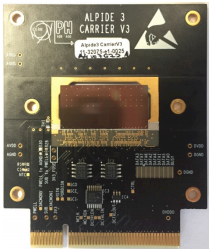
\includegraphics[width=100pt]{ALPIDE.png}
		\quad
		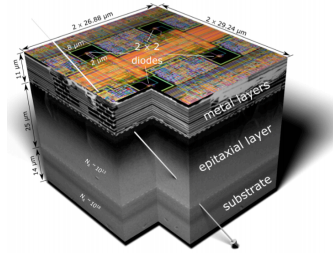
\includegraphics[width=140pt]{3D.png}
	    \end{figure}
    \end{itemize}
\end{frame}

\begin{frame}{The ALPIDE Telescope}
    \begin{figure}[H]
	\centering
	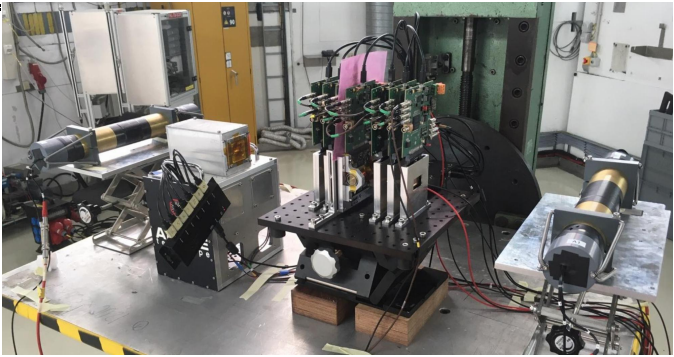
\includegraphics[width=\textwidth]{Telescope.png}
    \end{figure}
\end{frame}


\begin{frame}{Studies with the ALPIDE Telescope}
    \begin{minipage}{.44\textwidth}
	\LARGE Cosmics \normalsize \\
	\begin{itemize}
	    \item Event Plotting
		\begin{itemize}
		    \item \tiny Trying to create nice Looking (correctly scaled) 3D-
			Plots of cosmic tracks
		    \item Writing an Event oranizer for the huge amount of
			measurements performed
		\end{itemize}
	    \item Track analysis
		\begin{itemize}
		    \item \tiny Fitting lines to cosmics to determine valid and
			invalid tracks
		    \item \tiny Analyzing angular distribution
		    \item \tiny Comparison with Theoretical calcuations
		\end{itemize}
	    \item Plane Alignment
		\begin{itemize}
		    \item \tiny Using Tracks to align the Telescope  based on
			cosmic data
		    \item Comparing results to Testbeam Data from 2019 and 2020
		    \item Investigating differences in alignment after Transport
		\end{itemize}
	
	\end{itemize}
    \end{minipage}
    \begin{minipage}{.55\textwidth}
	\begin{figure}[H]
	    \centering
	    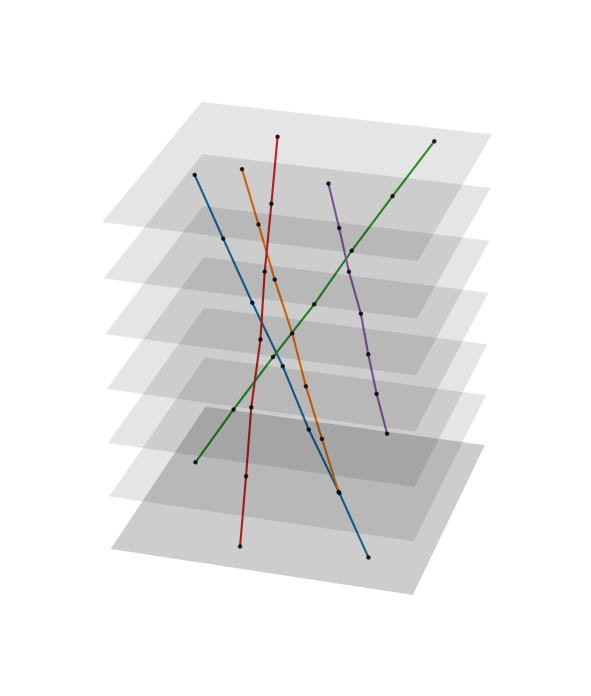
\includegraphics[width=\textwidth]{outlook.png}
	\end{figure}
    \end{minipage}
\end{frame}

\begin{frame}{Studies with the ALPIDE Telescope}
    \begin{figure}[H]
	\centering
	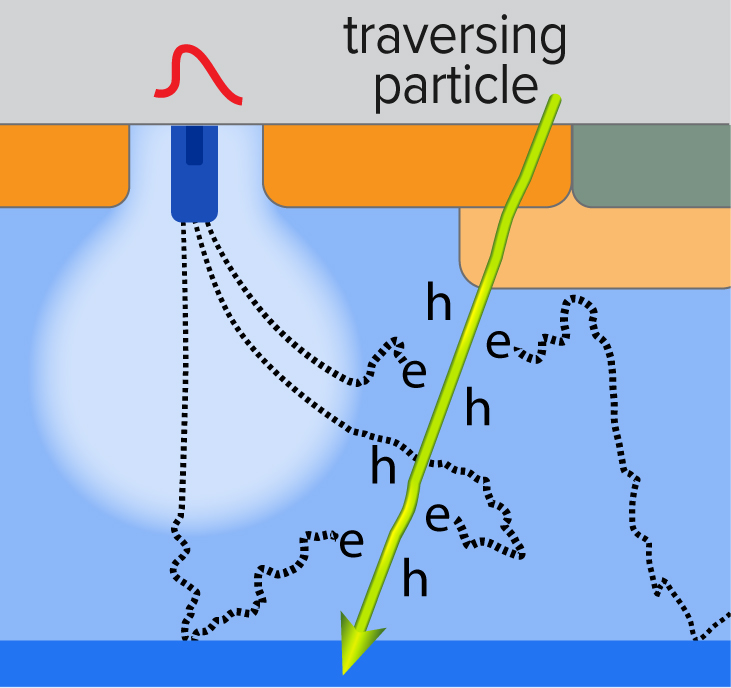
\includegraphics[width=.49\textwidth]{EH.jpg}
	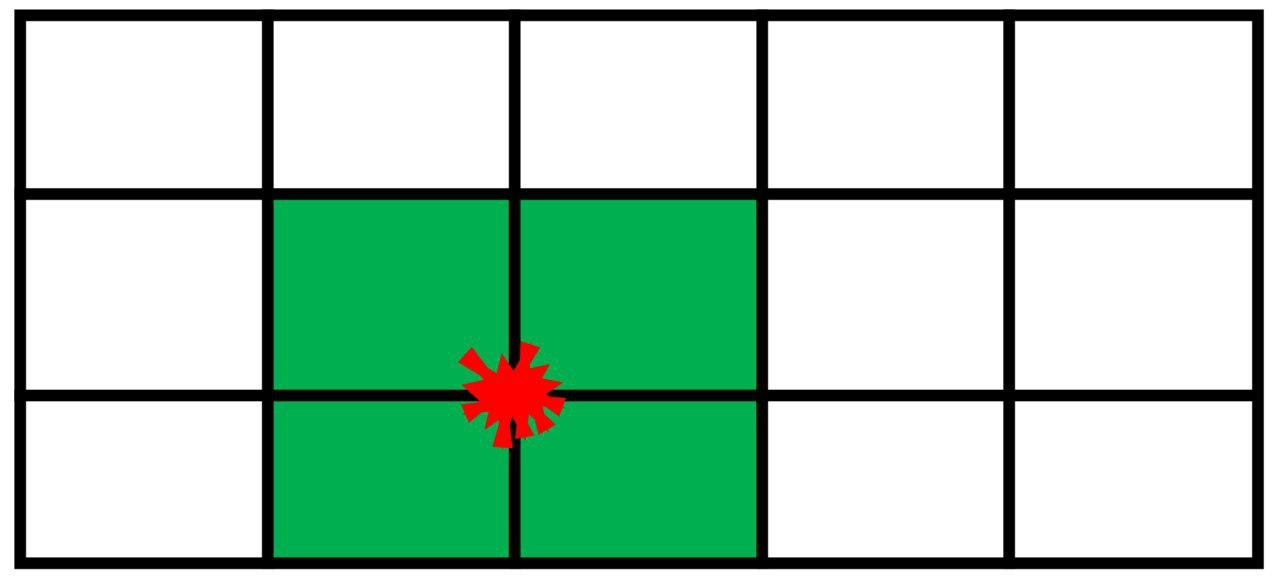
\includegraphics[width=.5\textwidth]{Davi.jpg}
\end{figure}
\end{frame}

\begin{frame}{Studies with the ALPIDE Telescope}
    \begin{figure}[H]
	\centering
	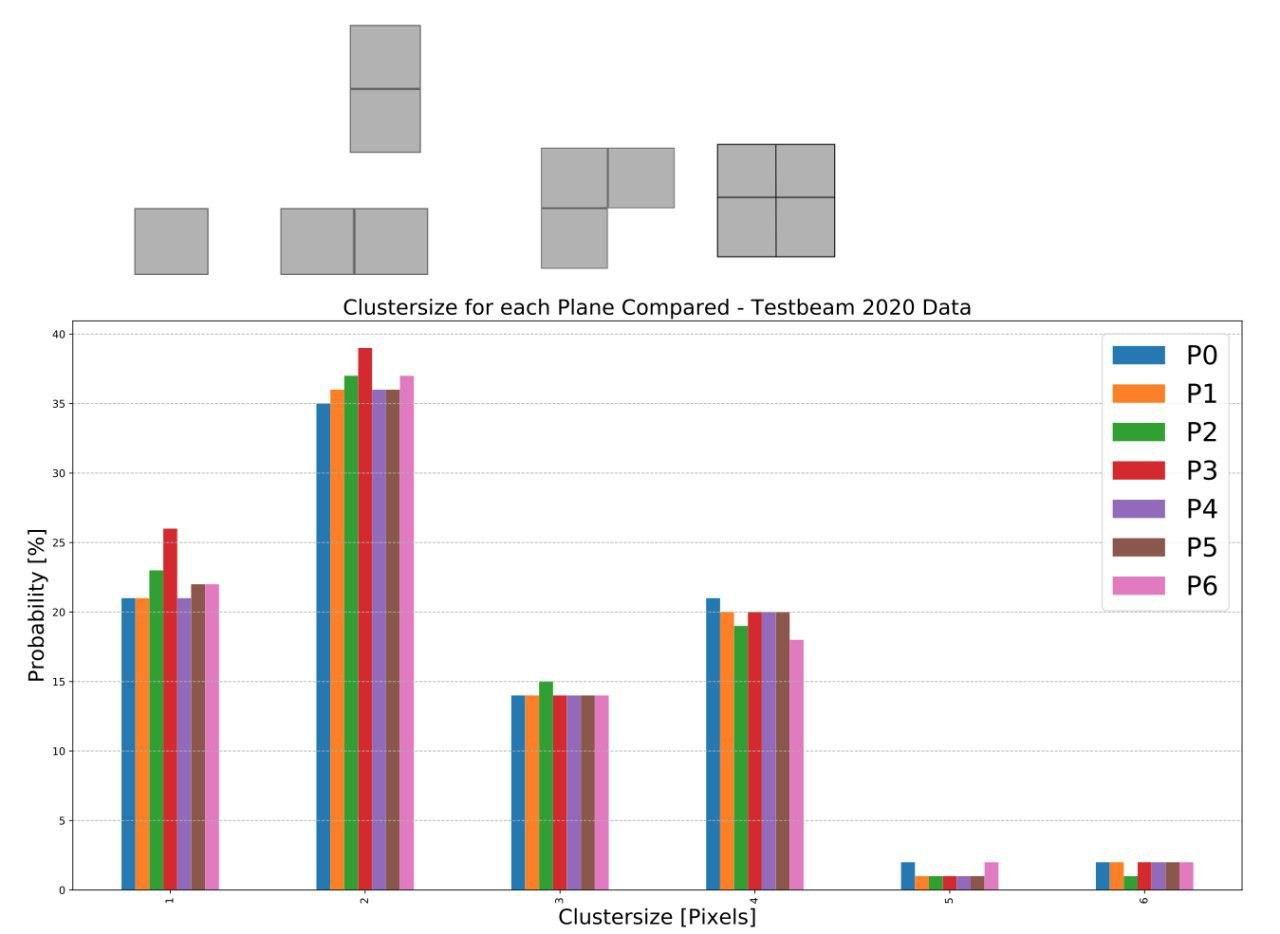
\includegraphics[width=.8\textwidth]{Feli2.jpg}
    \end{figure}
\end{frame}


\end{document}
